\section{Lastenheft zur Herstellung eines Gehäuses}
\subsection{Auftrag}
Es ist ein Gehäuse für den Signalgenerator herzustellen. Als Gehäuse wird ein Plastikgehäuse benutzt werden, welches bei dem Lieferanten Reichelt Elektronik\footnote{https://www.reichelt.de/} unter der Bestellnummer \glqq GEH KS 21\grqq\ zu bestellen ist. Der Gehäuseplan liegt diesem Lastenheft bei. Ebenfalls liegt eine Zeichnung mit den nötigen Modifikationen bei.

\subsection{Gehäuseplan}
\begin{center}
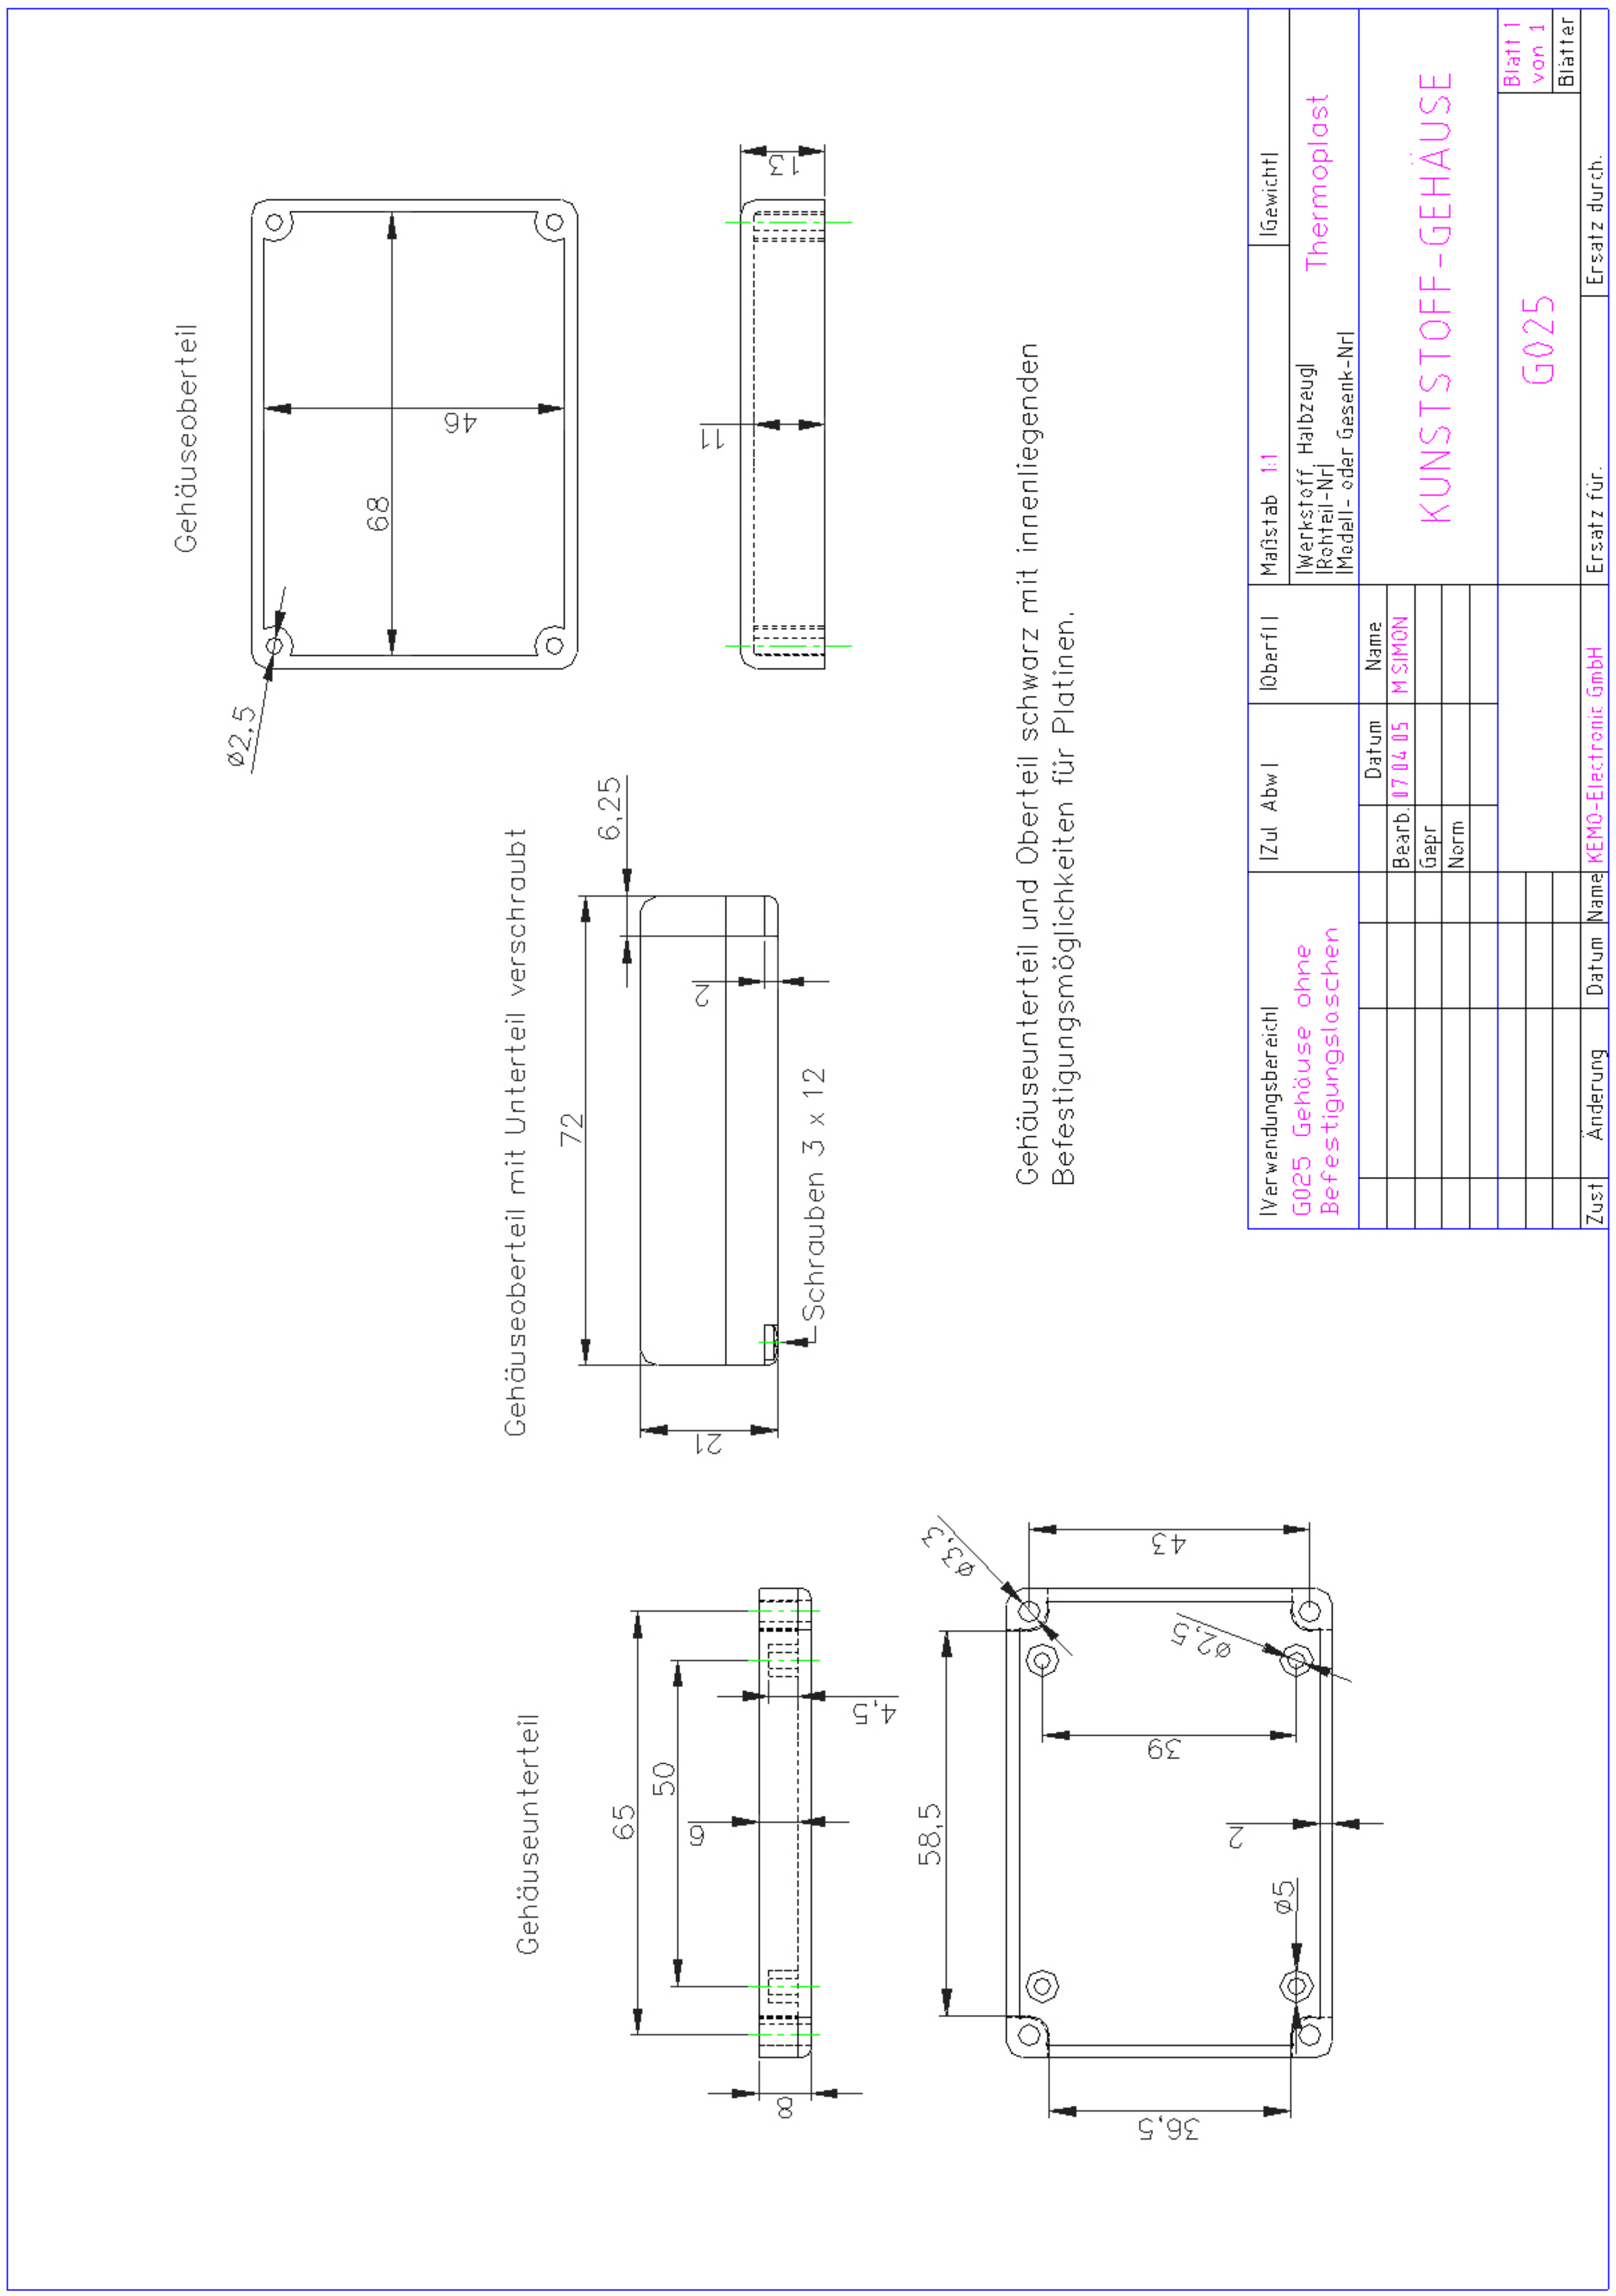
\includegraphics[width=0.8\textwidth]{./img/Gehauseplan.png}
\end{center}

\subsection{Änderungen am Gehäuse}
\begin{center}
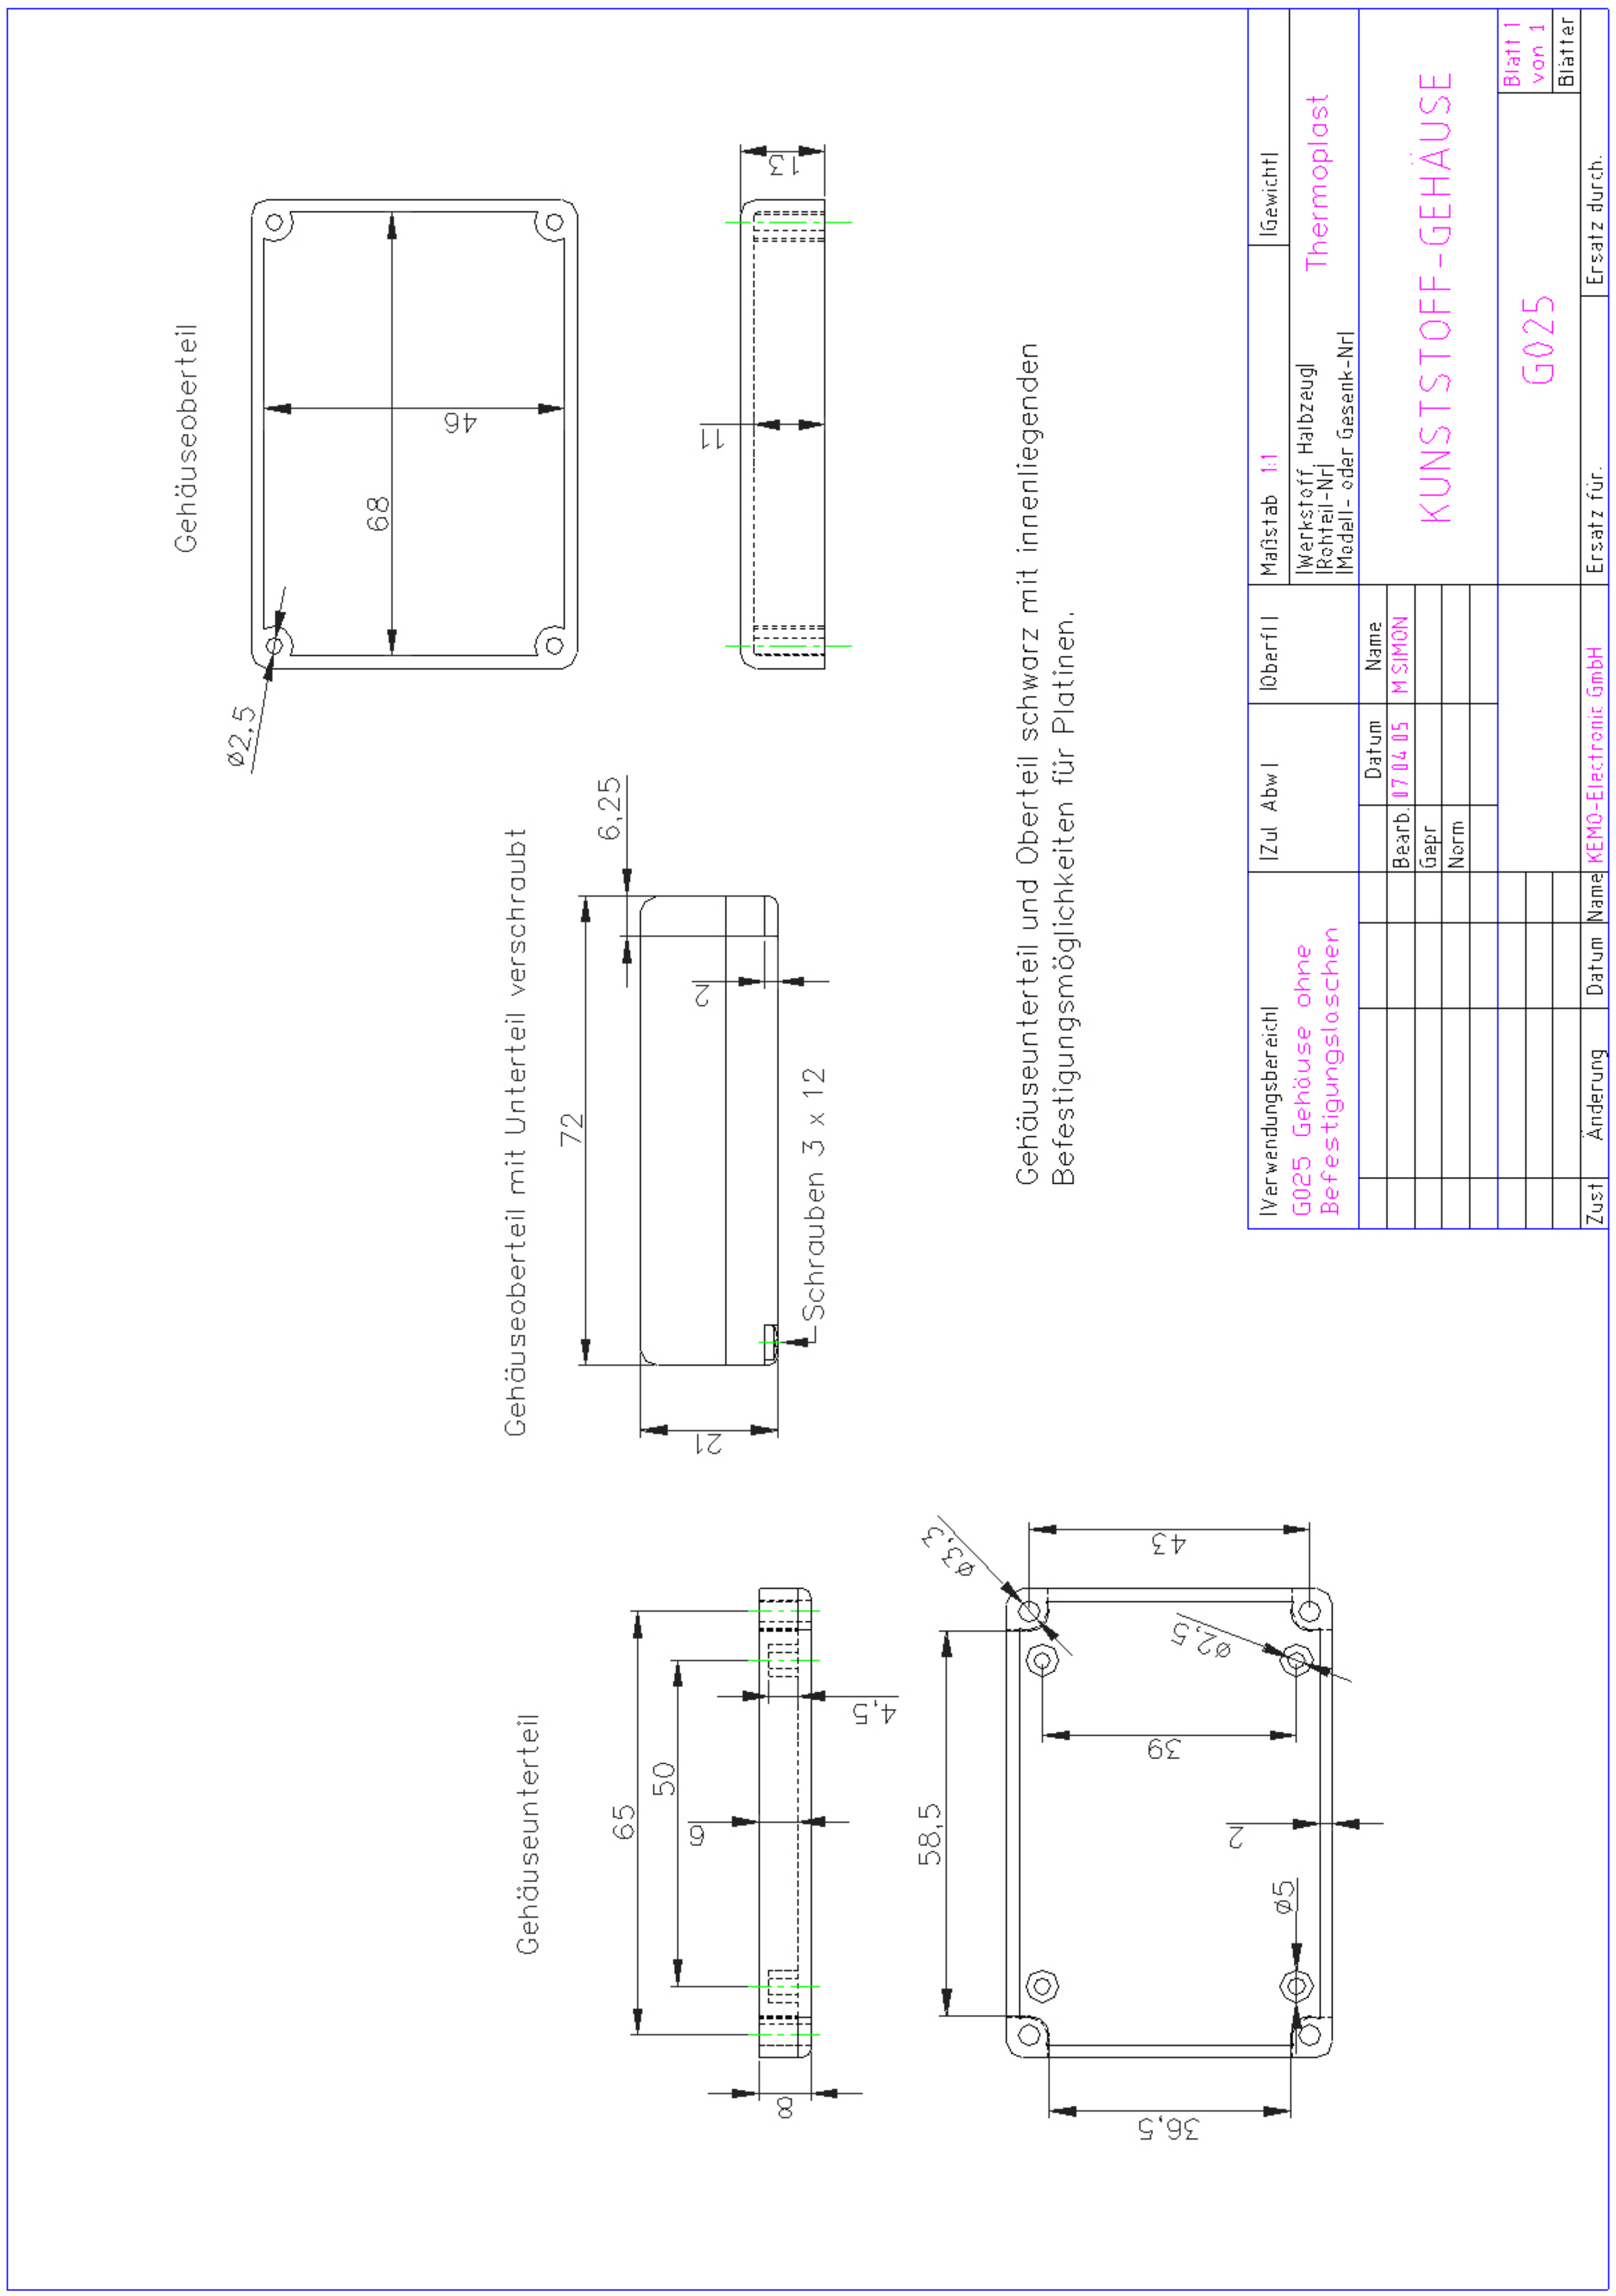
\includegraphics[width=\textwidth]{./img/GehauseAenderung.png}
\end{center}
